\section{Implementation}

\subsection{Probmal outline}
The goals it to turn the raw data from the \cams into an image format that can be passed to the \gls{h265} encoder, namely the \code{P010_10LE} format.
\code{P010_10LE} is a YCbCr 4:2:0 format with with semi-interlaced data and 10 bits per channel stored in the most significant bits of a 16 bit little-endian unsigned integers.

This involves separating different angles of polarization, debayering the byer data, translate the resulting RGB data to YcbCr, perform chroma subsampling and package the data in the correct way.
This whole process is visualzed in Figure \ref{fig:transform}.

\begin{figure}[H]
    \centering
    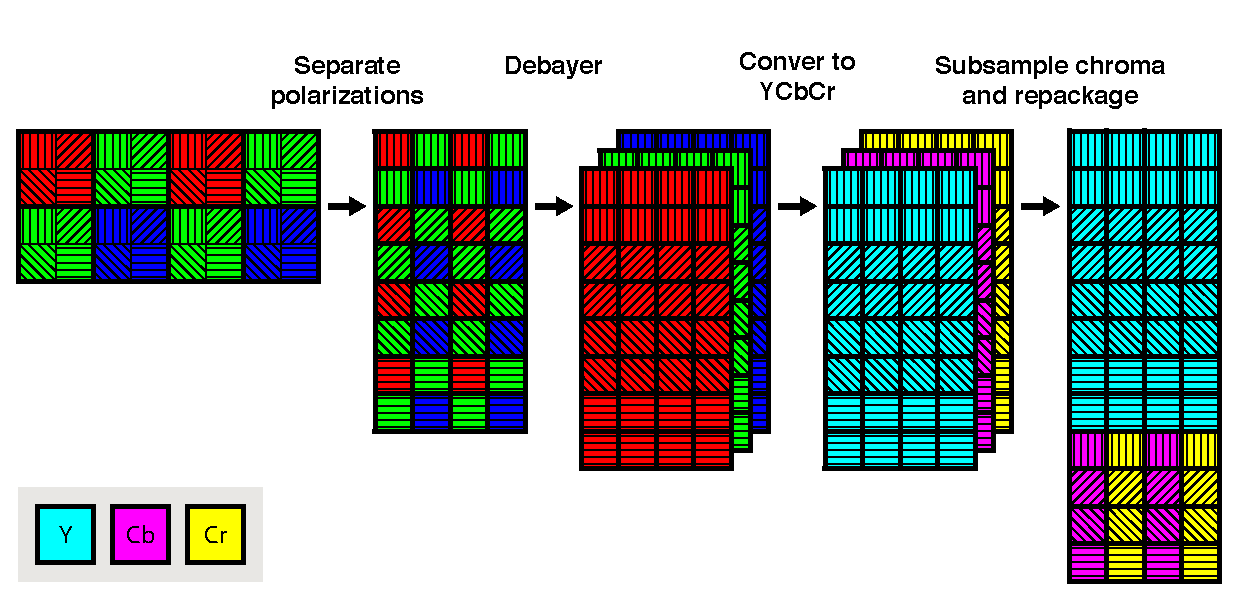
\includegraphics[width=\textwidth]{figures/polarized_image/transform.pdf}
    \caption{Visualization of how the raw custom bayer pattern is transforemd into a YCbCr format where the angles of polarization are stacked vertically.}
    \label{fig:transform}
\end{figure}

\begin{figure}[H]
    \centering
    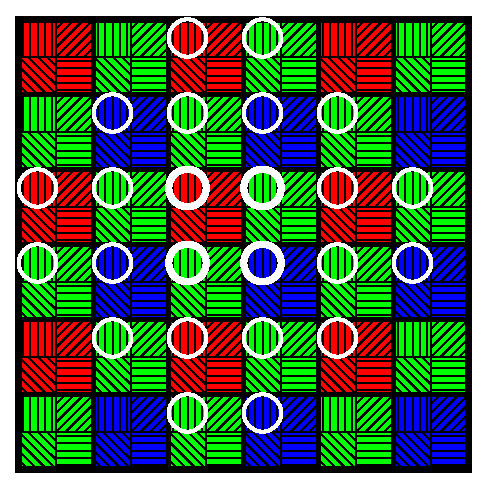
\includegraphics[width=.5\textwidth]{figures/polarized_image/normal_conv.pdf}
    \caption{Visualization of which pixels are used (white contour circle) to calculate the value of one Y value in the output image (filled white circle).}
    \label{fig:saperation}
\end{figure}


\begin{table}[H]
    \begin{minipage}[b]{.5\linewidth}
        \subcaptionbox{Separate debayering and color space conversion. Also shows where synchronization would be needed.}{
            \small
            \begin{tabular}{|l|c| c|}
                \hline
                \textbf{Operation}                         & \textbf{\# of \acrshort{fma}} \\
                \hline
                Green at red            (\ref{fig:mhc_gr}) & 9                             \\
                Green at blue           (\ref{fig:mhc_gb}) & 9                             \\
                Red at green 1 (\ref{fig:mhc_rgr})         & 11                            \\
                Red at green 2 (\ref{fig:mhc_rgb})         & 11                            \\
                Red at blue             (\ref{fig:mhc_rb}) & 9                             \\
                Blue at green 1 (\ref{fig:mhc_bgr})        & 11                            \\
                Blue at green 2 (\ref{fig:mhc_bgb})        & 11                            \\
                Blue at red             (\ref{fig:mhc_br}) & 9                             \\
                \textbf{\textit{Synchronize}}              &                               \\
                Convert to YCbCr                           & 36                            \\
                \textbf{\textit{Synchronize}}              &                               \\
                Binning Cb                                 & 4                             \\
                Binning Cr                                 & 4                             \\
                \hline
                \textbf{Total}                             & 124                           \\
                \hline
            \end{tabular}}
    \end{minipage}
    \begin{minipage}[b]{.5\linewidth}
        \subcaptionbox{Joined debayering and color space conversion.}{
            \small
            \begin{tabular}{|l|c|}
                \hline
                \textbf{Operation} & \textbf{\# of \acrshort{fma}} \\
                \hline
                Y at red           & 13                            \\
                Y at green 1       & 13                            \\
                Y at green 2       & 13                            \\
                Y at blue          & 13                            \\
                Cb                 & 24                            \\
                Cr                 & 24                            \\
                \hline
                \textbf{Total}     & 100                           \\
                \hline
            \end{tabular}}
    \end{minipage}
    \caption{Comparison of the number of \gls{fma} operations required to get the desired output. On the left }
\end{table}



\subsection{Efficient Separation}
The \gls{volta} has 48KiB of available shared memory per block \cite{rigerunNVIDIAJetsonXavier2023}.
With an image width of 2448 pixels \cite{lucidvisionlabsTriton0MPPolarization} it is only possible to store 10 lines in local shared memory.
\begin{align}
    \frac{48Kib}{2448px/line * 16b/px} = \frac{393216b}{39168b/l} \approx 10.039line
\end{align}

For simplicity we would want to store 12 rows or more in local memory to perform the debayering.


As a we want to dedicata parts of the local memory for preloading the next section while the current section is being processed, it is would not be possible to store
\begin{figure}[H]
    \centering
    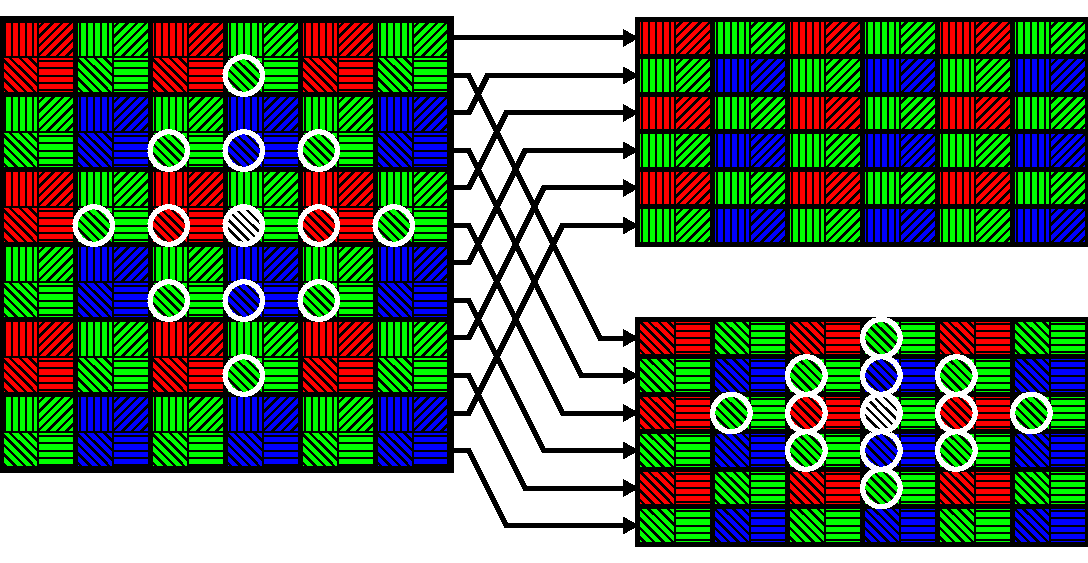
\includegraphics[width=\textwidth]{figures/polarized_image/separation.pdf}
    \caption{How separation is done in order to reduce amount of shared memory required per block.}
    \label{fig:saperation}
\end{figure}
Not problem on Orin.







With a runtime of $1 ms \pm 1 \mu s$
Nsight compute not working for memory











\subsection{Reuse optimization}
The current \gls{mhc} method requires six lines of the image to be available in local memory for efficient operation.
Techincally it woulb be possible to use only five, but this would result in more cumb

In order to efficiently

Another improvement was to use an array of pointers, rather than an array of arrays.
Initially the the section of the image on which calculations were performed were stored as an array of arrays in local shared memory.
When the computations on that part was performed, the whole block would move down.
\begin{figure}[H]
    \centering
    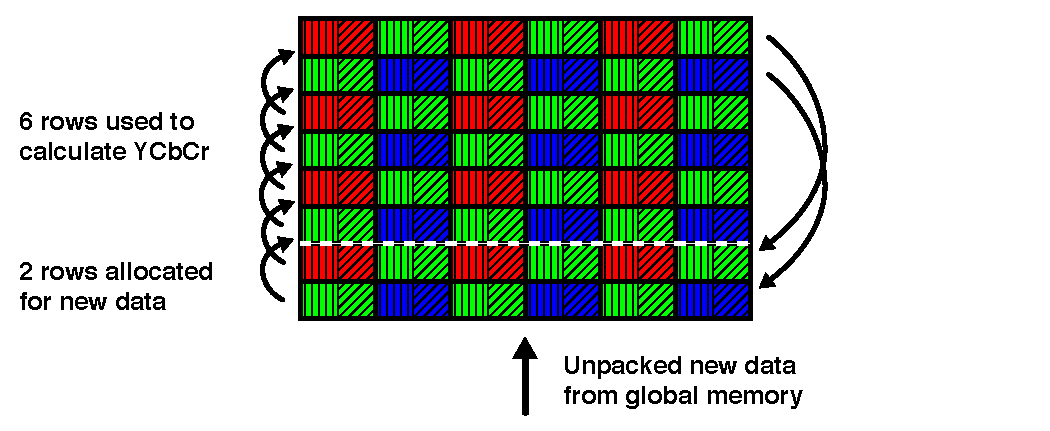
\includegraphics[width=\textwidth]{figures/polarized_image/rolling.pdf}
    \caption{TODO}
\end{figure}





\subsection{Half precitions floating point}